\documentclass{article}
\usepackage{amsmath}
\usepackage{graphicx}

\title{Winter Progress Report}
\date{}

\begin{document}

\maketitle

\section{Introduction}
This report will provide an overview of the progress made during the winter of 2024-2025. The report will cover the following topics:
\begin{itemize}
    \item Functional material to MCNP code and testing
    \item Previous and Upcoming Presentations
    \item Future Work
\end{itemize}

\section{Functional material to MCNP code and testing}
The functional material to MCNP code and testing was completed. The technique and code can be used to approximate varied soil compositions for simulations.
This is done so in a "cutting" method, where an MCNP geometry is divided into sections, enabling the definition of "varied" chemical compositions.

The following figures demonstrate the testing done:

First I describe a block of soil matching the dimensions of the soil in the most recent MINS architecture. 
I apply a function that describes the weight percentage of carbon in the soil. 
The function is a linear function of the depth of the soil. The function is as follows:

\[
f(z) =
\begin{cases} 
    C_0 + \frac{(C_1 - C_0)(z - z_0)}{z_1 - z_0}, & \text{for } z_0 \leq z \leq z_1, \\
    C_0, & \text{for } z \leq z_0, \\
    C_1, & \text{for } z \geq z_1.
\end{cases}
\]

with the following parameters:

\begin{itemize}
    \item $C_0 = 0.05$
    \item $C_1 = 0.25$
    \item $z_0 = 48$
    \item $z_1 = 48+45$
\end{itemize}

Here is a visual of the carbon content in the soil:

\begin{figure}[h]
    \centering
    \includegraphics[width=0.5\textwidth]{imgs/carbon_content.png}
    \caption{Carbon Content}
\end{figure}

The remaining elemental content is defined by a ratio:

\[
\begin{align*}
    \text{Nitrogen} &= 0.44 \times (1-\text{Carbon}) \\
    \text{Oxygen} &= 0.55 \times (1-\text{Carbon}) \\
    \text{Hydrogen} &= 0.01 \times (1-\text{Carbon})
\end{align*}
\]

The soil is separated into n sections, each with a different carbon content. Sampling the midpoint of each section, the materials are defined in MCNP. The following figures show the MCNP input geometry:

\begin{figure}[h]
    \centering
    \includegraphics[width=0.5\textwidth]{imgs/mcnp_geometry.png}
    \caption{MCNP Geometry}
\end{figure}

The input code for this can be located in atlas at /project/auburn-mins/andres/expirements/compute/soil_in_sections2 .

The materials carbon content at each slice level is shown in the following figure:

\begin{figure}[h]
    \centering
    \includegraphics[width=0.5\textwidth]{imgs/mcnp_carbon_content.png}
    \caption{MCNP Carbon Content}
\end{figure}

The MCNP code was run and the results are shown in the following figure:

\begin{figure}[h]
    \centering
    \includegraphics[width=0.5\textwidth]{imgs/mcnp_results.png}
    \caption{MCNP Results}
\end{figure}

Peak Fitting was done:

\begin{figure}[h]
    \centering
    \includegraphics[width=0.5\textwidth]{imgs/peak_fitting.png}
    \caption{Peak Fitting}
\end{figure}

On a graph, the peak areas vs sections are shown as follows:

\begin{figure}[h]
    \centering
    \includegraphics[width=0.5\textwidth]{imgs/peak_areas.png}
    \caption{Peak Areas}
\end{figure}

\section{Previous and Upcoming Presentations}

In the Fall I gave a poster presentation on the MINS project at a UTA conference "mathposium". 
The poster was well received and I was able to answer questions about the work.
The poster is attached to the email as this report.

Here is a picture of me presenting the poster:

\begin{figure}[h]
    \centering
    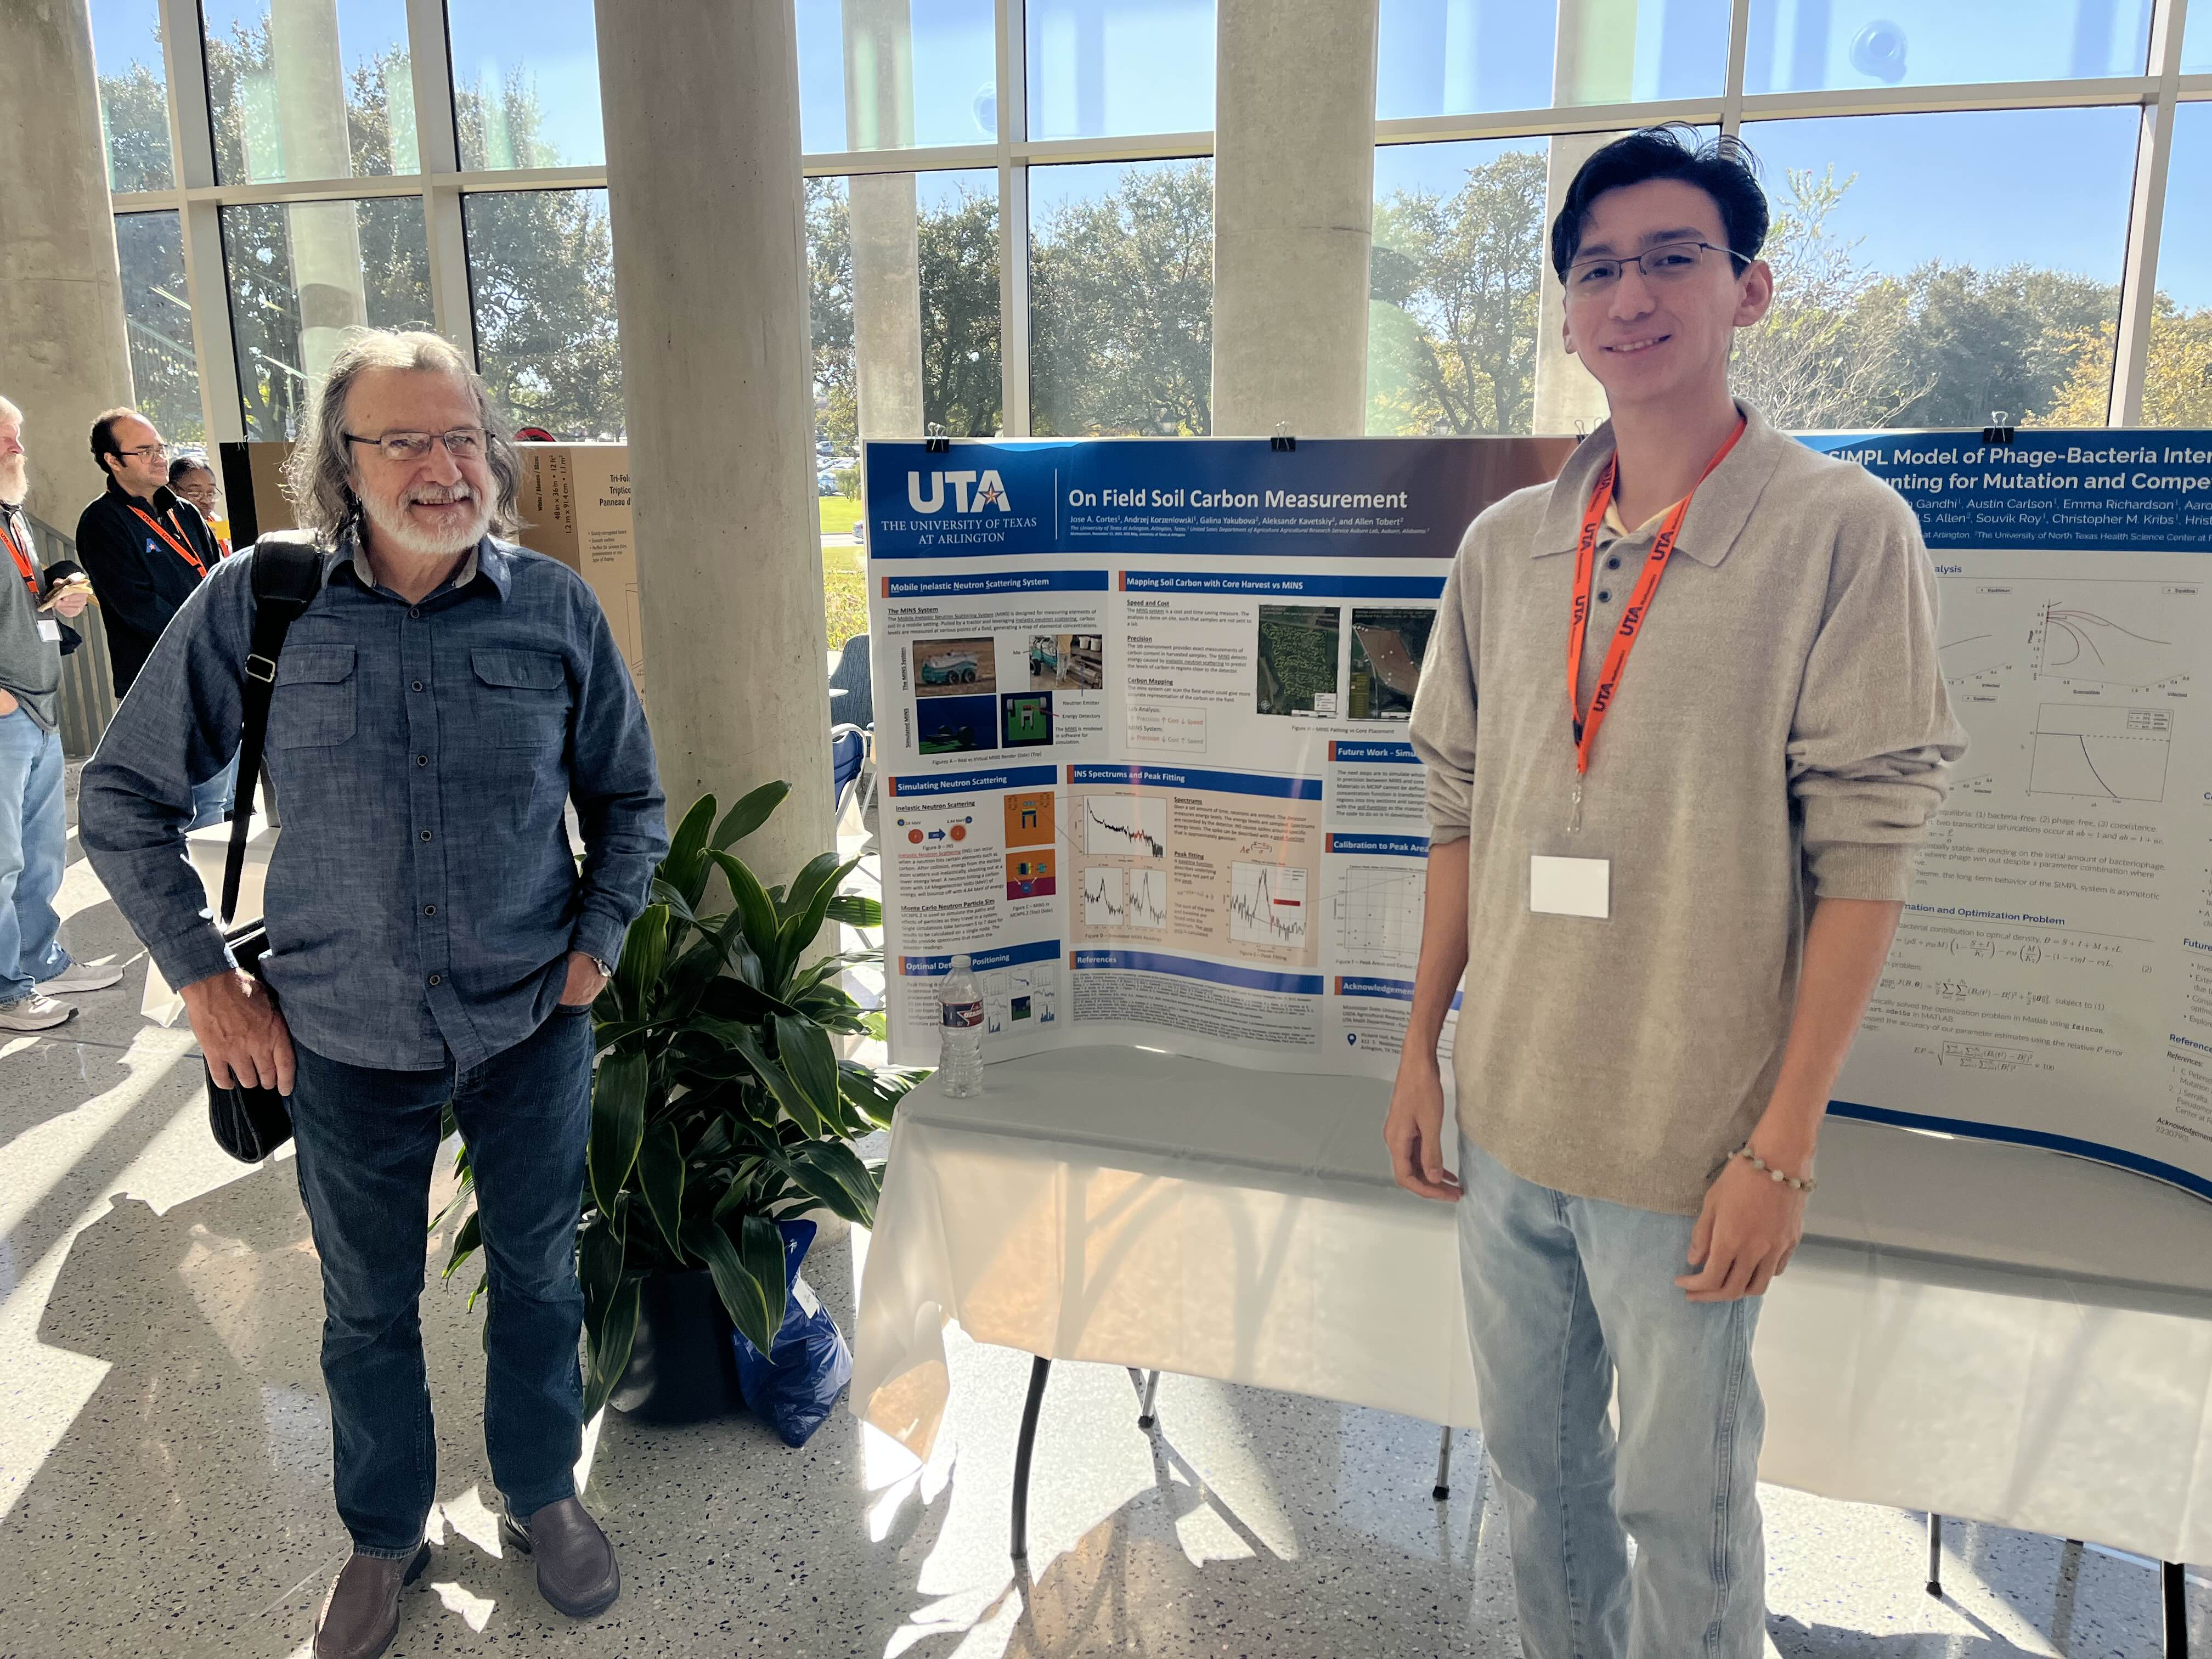
\includegraphics[width=0.5\textwidth]{imgs/image.png}
    \caption{Presentation}
\end{figure}

In the spring I hope to present at the Missouri State Conference on Agriculture and AI. 
There is a speaker and poster option, I am writing the abstract for the speaker option. 
Please let me know what you think of this. 

\section{Future Work}

\begin{itemize}
    \item Whole Field Simulation for comparison with cylinder harvest method
    \item Using the cutting method to generate f4 mesh in soil
\end{itemize}

\end{document}